\section{Codes and Initial Conditions}
\label{sec:c3_codes}

All hydrodynamic and magnetohydrodynamic codes seek to properly evolve the continuum dynamics of a fluid on a discrete set of points in space and time.  Most astrophysical fluid codes (including the two we use) explore the simpler regimes of ideal hydro- or magnetohydrodynamics, where molecular viscosity and electrical resistance are negligible, as such is generally the case in astrophysical settings outside of planetary interiors.  The coupled partial differential equations of ideal magnetohydrodynamics, in their conservative form and with Gaussian units (eg. \citealt{goedp04, pakms13, spru13}, \citealt{feidc12} Sec. 3), is

\begin{eqnarray}
\ptl_t\rho + \ptl_j(\rho u^j) &=& 0 \nonumber \\
\ptl_t(\rho u^i) + \ptl_j(\rho u^iu^j + \delta^{ij}P_\mrm{tot} - \frac{1}{4\pi}B^iB^j) &=& -\rho \ptl^i\Phi \nonumber \\
\ptl_t(\rho e) + \ptl^j\left(u_j (\rho e + P_\mrm{tot}) - \frac{B_j}{4\pi}(u^lB_l)\right) &=& -u_j\rho \ptl^j\Phi \nonumber \\
\ptl_t B^i + \ptl_j(u^jB^i - u^iB^j) &=& 0,
\label{eqn:c3_mhd_eqns}
\end{eqnarray}

\noindent where $\rho$, $u^i$, $B^i$, and $\Phi$ are the density, velocity, magnetic field and gravitational potential, respectively, $P_\mathrm{tot} = P + \frac{1}{8\pi}B_jB^j$ is the total pressure, $e = \frac{1}{2}u_iu^i + e_\mathrm{int} + \frac{1}{8\pi\rho}B_jB^j$ is the specific total energy, and the usual Einstein summation convention holds.  This can be written in compact form:

\eqbegin
\frac{\ptl {\bf U}}{\ptl t} + \nabla\cdot{\bf F(U)} = {\bf G}
\label{eqn:c3_mhd_eqns_compact}
\eqend

\noindent where

\eqbegin
{\bf U} = 
\left( \begin{array}{c}
\rho \\
\rho {\bf u} \\
\rho e \\
{\bf B} \end{array} \right),
\label{eqn:c3_mhd_eqns_u}
\eqend

\eqbegin
{\bf F(U)} = 
\left( \begin{array}{c}
\rho {\bf u} \\
\rho {\bf u}{\bf u}^T + P_\mathrm{tot} - \frac{1}{4\pi}{\bf B}{\bf B}^T \\
{\bf u} (e + P_\mathrm{tot}) - \frac{{\bf B}}{4\pi}({\bf u}\cdot{\bf B}) \\
{\bf B}{\bf u}^T - {\bf u}{\bf B}^T\end{array} \right),
\label{eqn:c3_mhd_eqns_fu}
\eqend

\eqbegin
{\bf G} = 
\left( \begin{array}{c}
0 \\
\rho {\bf g} \\
\rho {\bf u}\cdot {\bf g} \\
0 \end{array} \right)
\label{eqn:c3_mhd_eqns_g},
\eqend

\noindent and ${\bf g} = -\nabla\Phi$ is the gravitational acceleration.  Eqn. \ref{eqn:c3_mhd_eqns_compact} shows that the time-derivative of the fluid's values is given by the sum of a flux term (since, by the Green-Gauss theorem, the integral of $\nabla\cdot{\bf F(U)}$ within a volume is equivalent to a flux across its boundary) and a (self-)gravitational source term ${\bf G}$.  These are generally calculated separately, and then combined.

To better understand the code comparison in this chapter, and to preface the discussion of improving \arepo's angular momentum conservation in Sec. \ref{sec:c3_fixingarepo}, we present an extremely short and semi-qualitative discussion of how these equations are implemented within SPH and \arepo.  The historical development of both methods is long and involved, and, as improving hydrodynamic simulations is not the focus of this thesis, we will refer the reader to a number review articles referenced throughout this section for further details.

\subsection{Traditional Smoothed-Particle Hydrodynamics}
\label{ssec:c3_sph}

SPH, first introduced in \cite{lucy77} and \cite{gingm77}, is a mature simulation method used in a host of astrophysical contexts ranging from star formation to cosmology.  Our overview summarizes the first few sections of \citep{spri10rev}; we also refer readers to \cite{mona05} and \cite{ross09} for further details.

SPH represents a fluid with a set of particles.  The fluid's continuum properties at some point ${\bf r}$ in the simulation are sampled by using these particles as interpolation points.  Representing any given continuum property (the most important of which is density, since it factors into the equations of motion) as $F({\bf r})$, we can use a ``kernel'' $W({\bf r}, h)$ to generate its approximate, locally-averaged value

\eqbegin
F_s({\bf r}) = \int F({\bf r'})W({\bf r} - {\bf r'}, h)d{\bf r'}.
\eqend

\noindent In the (computationally impossible) case of infinite resolution, we can choose $W({\bf r}, h)$ to be a Dirac delta, and $F_s({\bf r}) = F({\bf r})$, but in practice we choose $W({\bf r}, h)$ to extend over some characteristic ``smoothing length'' $h$.  If $W({\bf r}, h)$ were a Gaussian, $h = \sigma$, the standard deviation.  The most popular form of $W({\bf r}, h)$ is a cubic spline that goes to zero when ${\bf r} > 2h$, and $h$ is generally set to ensure a user-defined number of neighboring particles $N$ fall within the kernel.  For a set of particles with associated mass $m_i$ and known values of $F_i = F({\bf r}_i)$, we can discretize the integral as

\eqbegin
F_s({\bf r}) = \sum_j\frac{m_j}{\rho_j}F_j W({\bf r} - {\bf r}_j, h).
\label{eq:c3_kernelavg}
\eqend

\noindent where $\rho_i$ can be estimated using 

\eqbegin
\rho_i = \sum_j m_j W({\bf r}_i - {\bf r}_j, h)
\label{eq:c3_kernelavg_rho}
\eqend

\noindent Derivatives of the field can also be determined using the gradient of the kernel $\nabla_i W_{ij}$.

Meanwhile, the Euler equations (Eqn. \ref{eqn:c3_mhd_eqns_compact} without the gravitational and magnetic terms) can be shown to follow the Lagrangian:

\eqbegin
L = \int \rho\left(\frac{{\bf u}^2}{2} - e\right)dV
\label{eqn:c3_lagrangian}
\eqend

\noindent which can be discretized for a set of particles as

\eqbegin
L_\mathrm{SPH} = \sum_i \frac{1}{2}m_i u_i^2 - m_i e_i.
\eqend

\noindent This suggests a time-evolution scheme for the fluid.  Each particle representing the fluid is given a (time-independent) mass $m_i$, position ${\bf r}_i$, velocity ${\bf u}_i$ and specific internal energy $e_i$; the fluid can then be simulated by time-evolving the latter three terms for all particles.  The equations governing ${\bf u}_i$ and $e_i$ are derived by applying the Euler-Lagrange equation ($\frac{d}{dt}\frac{\ptl L}{\ptl \dot{{\bf r}}_i} - \frac{\ptl L}{\ptl {\bf r}_i} = 0$) to $L_\mathrm{SPH}$.  They traditionally take the form:\footnote{We state \cite{wadssq04}'s formulation of Eqns. \ref{eqn:c3_spheqnm} and \ref{eqn:c3_spheqne}, as \cite{spri10rev} assumes a different method of controlling the smoothing length $h_i$.}

\eqbegin
\frac{d{\bf u}_i}{dt} = -\sum_j m_j\left(\frac{P_i}{\rho_i^2} + \frac{P_j}{\rho_j^2} \right)\nabla_i W_{ij}
\label{eqn:c3_spheqnm}
\eqend

\eqbegin
\frac{d e_i}{dt} = \frac{P_i}{\rho_i^2}\sum_j m_j\left({\bf u}_{i} - {\bf u}_{j}\right)\cdot\nabla_i W_{ij}
\label{eqn:c3_spheqne}
\eqend

\noindent where pressure $P_i$ is determined from $\rho_i$ and $e_i$ using a user-prescribed equation of state.  The left panel of Fig. \ref{fig:c3_codediag} summarizes this scheme.  Note that since Eqn. \ref{eqn:c3_lagrangian} has no time-dependence and is translationally and rotationally invariant, SPH naturally conserves total energy, momentum and angular momentum.  Self-gravity can be added as an additional force to Eqn. \ref{eqn:c3_spheqnm} (see \citealt{spri10rev}, Sec. 2.4, and \citealt{wadssq04}, Sec. 2.1) using methods originally developed for $N$-body simulations.  Magnetic fields can also be included (eg. \citealt{pric12, lewibt16}), but the resulting ``SPHMHD'' formulation is not used in this thesis.

% Eqn. \ref{eqn:c3_spheqne} can actually be replaced with $d s_i/dt = 0$, except in the presence of shocks

%(as the differential form of the Euler equations breaks down across a shock front)

As given, the SPH equations of motion conserve entropy, but entropy must increase in the presence of shocks.  The most popular solution is to add an artificial viscosity term

\eqbegin
-\sum_j m_j \Pi_{ij} \nabla_i W_{ij}
\eqend

\noindent to Eqn. \ref{eqn:c3_spheqnm}, where, defining ${\bf r}_{ij} = {\bf r}_i - {\bf r}_j$ and ${\bf u}_{ij} = {\bf u}_i - {\bf u}_j$,

\eqbegin
\Pi_{ij} =
    \begin{cases}
      \frac{-\alpha\frac{1}{2}(c_i + c_j)\mu_{ij} + \beta\mu_{ij}^2}{\frac{1}{2}(\rho_i + \rho_j)} & \mrm{for\,} {\bf u}_{ij}\cdot{\bf r}_{ij} < 0 \\
      0 & \mrm{otherwise},
    \end{cases}
\label{eq:c3_artificialvisc}
\eqend

\noindent where $\mu_{ij} = \bar{h}{\bf u}_{ij}\cdot{\bf r}_{ij}/(|{\bf r}_{ij}|^2 + 0.04\bar{h}^2)$, $\bar{h} = \frac{1}{2}(h_i + h_j)$, $c_i$ is the sound speed and $\alpha$ and $\beta$ are tunable parameters ($\beta = 2\alpha$ is used in \gasoline).  In addition to facilitating shock capture, $\Pi_{ij}$ also prevents spurious particle interpenetration between interacting flows \citep{hernk89}.  It, however, can also introduce spurious viscous forces, and so must be damped in the absence of shocks.  In shear flows, this can be done with a ``Balsara switch'', which multiplies $\Pi_{ij}$ with a prefactor, proportional to the ratio between the divergence and curl of velocity, that goes to zero in the presence of a pure shear flow.  It is also possible to make the $\alpha$ and $\beta$ coefficients in $\Pi_{ij}$ time-variable (eg. \citealt{morrm97, dola+05}) with

\eqbegin
\frac{d\alpha_i}{dt} = -\frac{\alpha_i - \alpha_\mrm{min}}{\tau_i} + S_i
\label{eq:c3_timevariablealpha}
\eqend

\noindent where $\tau_i = h_i/(c_i l)$, $l$ is a tuneable parameter of order unity, $S_i$ is a source term that becomes large in the prescence of shocks, and $\alpha_\mrm{min} > 0$ is a minimum $\alpha$ value to negate noise and spurious particle interpenetration in smooth flows.  Eqn. \ref{eq:c3_timevariablealpha} exponentially damps $\alpha_i$ to its minimum value over timescale $\tau_i$ in the absence of shocks, and increases it via the source term when shocks are present.  Both these methods are used in \gasoline.

%{eq:c3_artificialvisc}

As explained in the introduction, SPH's Lagrangian nature allows it to automatically resolve regions of high density, simulate advection without errors, and conserve energy, linear and angular momentum to high accuracy.  These features make it much easier to model mergers in SPH than in Eulerian grid schemes, which discretize the simulation volume on a static grid, and time-evolve the system by tracking fluid fluxes between grid cells.  These traditionally have issues with simulating advection and adaptively increasing the spatial resolution ahead of moving fluids, such as orbiting binary stars, except under specific coordinate systems and symmetries.  Thus, they have rarely been used to simulate WD mergers (see \cite{katz+16} for recent developments).

The limitations of SPH (and Eulerian codes) have also been well-covered in literature (see, eg., the introductions to \citealt{spri10, hopk15, katz+16}).  Chief among them is the artificial viscosity discussed above, which can produce spurious heating and angular momentum transport in shear flows even in codes that utilize the Balsara switch and time-variable viscosity \citep{culld10}.  Classical formulations of SPH have also been known to suppress hydrodynamic instabilties (eg. \citealt{ager+07}) due to poor treatment of contact discontinuities manifesting as a ``surface tension'' (eg. \citealt{readha10, hesss10}).  While this has subsequently been resolved (eg. \citealt{hopk13, hu+14, kell+14}) by introducing artificial mixing terms \citep{pric08} and smoothing the pressure as well as the density across discontinuities (eg. by replacing the $P_i/\rho_i^2 + P_j/\rho_j^2$ term in Eqn. \ref{eqn:c3_spheqnm} with $(P_i + P_j)/(\rho_i\rho_j)$; \citealt{kell+14}) the vast majority of merger simulations in the literature come from before these alterations became widely used.  SPH resolves shocks and steep gradients relatively poorly compared to Eulerian schemes due to kernel smoothing of the density, and can corrupt smooth flows with particle velocity noise \citep{spri10rev}.  Lastly, SPH particles naturally tend toward a locally isotropic and regular configuration \citep{pric12}, and in physical systems where they are irregularly distributed, such as in shear flows and after shocks, Eqn. \ref{eqn:c3_spheqnm} produces spurious forces to restore regularity (eg. \citealt{readha10, dehna12}).  In some situations, this resolution-independent ``$E_0$ error'' produces enough noise to drown out large-scale structures \citep{hopk15}.  All of these issues motivate both the further development of SPH and competing hydrodynamic schemes, and simulating mergers in a diversity of codes.

%the E0 error also contributes to poor treatment of discontinuities; 

\subsection{GASOLINE SPH Code}
\label{ssec:c3_gasoline}

\gasoline\ is a modular, tree-based SPH code that we previously used to explore the parameter space of CO WD mergers in Ch. \ref{ch:ch2}.  Code settings and initial conditions used in this work are nearly identical to those used in Ch. \ref{ch:ch2}.  We utilize \gasoline's default \cite{hernk89} kernel with 100 neighbours, and use the asymmetric energy formulation (\citeauthor{wadssq04} Eqn. 8) to evolve particle internal energy.  Artificial viscosity is dynamically controlled using a combination of the Balsara switch and time-variable coefficients for the $\alpha$ and $\beta$ viscosity terms ($\alpha\,=0.05$, $\beta\,=0.1$ when shocks are not present, and approximately unity when they are).  We utilize the Helmholtz equation of state (EOS; \citealt{timms00}) to properly represent arbitrarily degenerate and relativistic gases.  Since \gasoline\ tracks the particle internal energy, while Helmholtz uses temperature as an input, a Newton-Raphson inverter is included in the EOS to determine the latter from the former.  To keep the energy-temperature relation positive-definite for the inverter, we enable Coulomb corrections even when the total entropy becomes negative.  SPH noise ocassionally brings highly degenerate particles to below the Fermi energy.  Under these conditions we set the pressure to the Fermi pressure, but let the energy freely evolve (see Sec. \ref{ssec:c2_sphcode}).

Like in our previous work, we ignore outer hydrogen and helium layers, composition gradients, and any nuclear reactions, in order to focus on the merger hydrodynamics.  Previous work that did include nuclear reactions \citep{loreig09,dan+12}, and in one case an outer helium layer \citep{rask+12}, have shown that they play a negligible role in the hydrodynamics of a $0.625 - 0.65\,\Msun$ CO WD merger.  More massive binaries, as well as less massive ones involving a CO-He hybrid WD, may experience He or CO detonantions during the merger \citep{pakm+10, rask+12, dan+12, pakm+13}.

We use the same version of \gasoline\ as in Ch. \ref{ch:ch2}, which does not include the improvements recently introduced in \textsc{Gasoline2} \citep{kell+15, tamb+15} and \textsc{ChaNGa/Gasoline} \citep{gove+15}.  These include a turbulent diffusion scheme to facilitate fluid mixing \citep{shen+10} and the use of the $(P_i + P_j)/(\rho_i\rho_j)$ density-averaged pressure term in the SPH force expression \citep{kell+14} to properly treat contact discontinuities.  We also do not consider more advanced prescriptions for viscosity, such as Godunov-SPH (eg. \citealt{chaw16}), as these are generally not implemented in SPH codes.  We again stress that the purpose of this work is to compare the traditional SPH formulation, used in almost all merger simulations to date, to \arepo, and we leave comparisons with improved and modified SPH schemes to future work.

%kell+14 is practically equivalent to the pressure-entropy formulation of \cite{hopk13})

\subsection{AREPO Moving Mesh Code}
\label{ssec:c3_arepo}

\begin{figure}
\centering
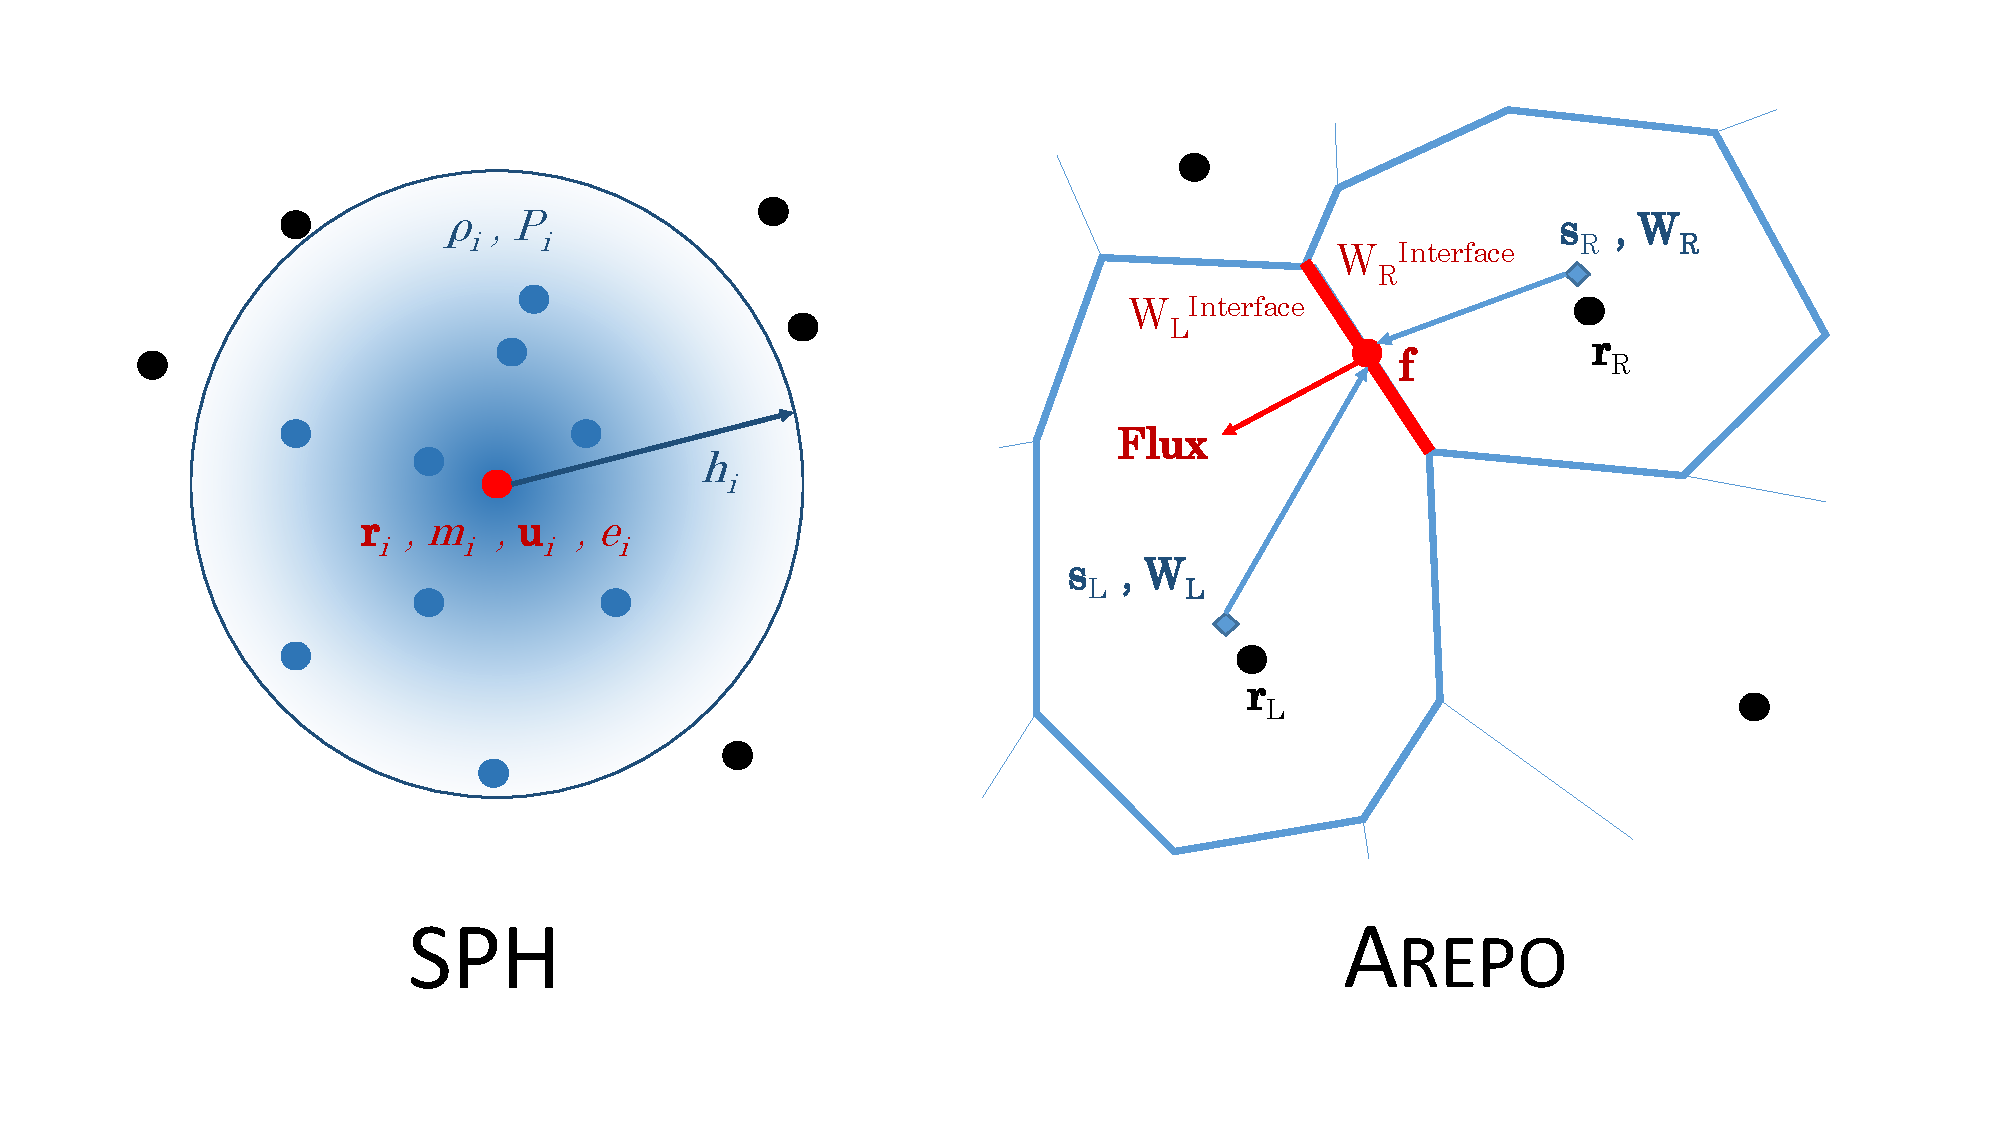
\includegraphics[angle=0,width=1.0\columnwidth]{chapter3_zhu+u/figures/SPHArepoFig.pdf}
\caption{Schematics for the SPH and \arepo\ hydrodynamic schemes.  In SPH (left), the fluid is discretized into particles, each of which possesses a position ${\bf r}_i$, mass $m_i$, velocity ${\bf u}_i$ and specific internal energy $e_i$.  The density $\rho_i$ of a given particle (red point) is determined by kernel sampling its neighbors (blue) within a smoothing length $h_i$ (Eqn. \ref{eq:c3_kernelavg_rho}); pressure $P_i$ is then obtained using the density and internal energy.  The particle is evolved by kernel sampling nearby pressures and densities, and applying the SPH equations of motion (Eqns. \ref{eqn:c3_spheqnm} and \ref{eqn:c3_spheqne}).  In \arepo\ (right), the fluid is discretized using an unstructured mesh defined by Voronoi tessellation.  Each Voronoi cell possesses a mesh-generating point ${\bf r}_i$ and a set of conserved quantities equivalent to ``primitive variables'' ${\bf W}_i = \left(\rho_i, {\bf u}_i, P_i, {\bf B}_i\right)$, i.e. the values of density, velocity, pressure and magnetic field amplitude at the cell's center of mass ${\bf s}_i$.  Note that ${\bf r}_i \neq {\bf s}_i$, but their separation is typically a few percent of the cell's radius, and has been exaggerated above.  Fluxes between two cells $\mrm{L}$ and $\mrm{R}$ are calculated by propagating their primitive variables ${\bf W}_\mrm{L,R}$ to the centroid of their interface ${\bf f}$ to obtain ${\bf W}_\mrm{L,R}^\mrm{interface}$ (Eqn. \ref{eq:c3_muscl_hancock}, or Eqn. \ref{eq:c3_rk2_timeevo} following \citealt{pakm+16}), and then solving the Riemann problem (in the frame of the interface).  The mesh is evolved by moving the mesh generating points ${\bf r}_i$ at roughly the fluid velocity ${\bf u}_i$, calculating fluxes between all cells, and then updating each cell's conserved quantities.  While evolving an SPH particle requires the use of dozens of its neighbors for kernel averaging, evolving an \arepo\ cell only requires those neighbors directly adjacent to it.}
\label{fig:c3_codediag}
\end{figure}

We now introduce \arepo's moving-mesh magnetohydrodynamics scheme, summarizing \cite{spri10}, \cite{pakmbs11} and \cite{pakms13}.  \arepo\ discretizes a fluid using a mesh (i.e. a grid), much like static Eulerian codes.  To overcome the traditional Eulerian code shortcomings of not being Galilean invariant, having large advection errors and having difficulty adjusting spatial resolution for complex flows, \arepo\ moves the mesh to follow local fluid motion.  Fluxes between mesh cells are calculated in the frame of the (moving) cell walls that divide them -- this preferred frame choice, in addition to the moving mesh, give the scheme a Lagrangian nature and automatic spatial refinement similar to SPH.  Allowing a structured grid to move with the fluid can lead to severe mesh deformation that prevent its further evolution.  \arepo\ circumvents this by utilizing an unstructured mesh defined by Voronoi tessellation (see \citealt{spri10}, Sec. 2) of a set of ``mesh-generating points'', each of which corresponds to a single mesh cell.  The mesh-generating points are given the velocities of the fluid they represent, and the tessellation is redone at each timestep.  The result is a moving mesh that, due to the mathematical properties of Voronoi tessellation, does not suffer from mesh-tangling effects.  To keep the Voronoi mesh regular (improving computational efficiency), mesh-generating point velocities are slightly altered from their pure Lagrangian values, and additional velocity adjustments can be made to keep cells near a constant mass or volume.  This representation of the fluid also couples more naturally to $N$-body based gravity solvers (see \citealt{spri10}, Sec. 3), with \arepo\ using a nearly identical TreePM solver as the SPH code \textsc{gadget2} \citep{spri05}.

%The mesh is constructed by Voronoi tesselation of a set of mesh generating points, and these points are given velocities to follow local fluid motion in a Lagrangian fashion.  This results in a mesh that deforms over time to track the evolution of the fluid, without the mesh-tangling effects that hindered previous moving mesh schemes.  Mesh generating point velocities are slightly altered from their pure Lagrangian values to keep the Voronoi mesh regular, reducing flux calculation errors.  Additional velocity adjustments can be made to keep cells near a constant mass or volume, but in practice this becomes ineffective for highly non-linear flows.  Fluid fluxes between cells are calculated using a second-order Godunov scheme with an exact Riemann solver (in our case HLLD), while self-gravity is handled using a TreePM solver, nearly identical to the one used by SPH code \textsc{gadget2} \citep{spri05}.

On the Voronoi mesh, \arepo\ tracks the finite volume integral of ${\bf U}$ (Eqn. \ref{eqn:c3_mhd_eqns_u}) for each cell, i.e. 

\eqbegin
{\bf Q}_i = \int_{V_i} {\bf U}dV = \left( \begin{array}{c}
m_i \\
{\bf p}_i \\
E_i \\
{\bf B}_i V_i \end{array} \right),
\eqend

\noindent where $m_i$ is the cell mass, ${\bf p}_i$ its momentum, $E_i$ its total energy and ${\bf B}_i V_i$ the magnetic field multiplied by the cell volume.  The time-evolution for cell $i$ from timestep $n$ to $n+1$ is then given by

\eqbegin
{\bf Q}_i^{n+1} = {\bf Q}_i^n - \Delta t\sum_j A_{ij} {\bf \hat{F}}_{ij}^{n + 1/2}
\label{eq:c3_arepo_timeadv}
\eqend

\noindent where $\Delta t$ is the timestep, $j$ stands for all cells that border cell $i$, $A_{ij}$ is the oriented area of the face dividing cells $i$ and $j$ and ${\bf \hat{F}}_{ij}$ is the estimated flux between them (positive flux means escaping from $i$).  In practice fluxes are more easily calculated using primitive variables 

% They're more easily calculated because of the Galilean transforms needed to determine cell fluxes, and to make self-gravity easier to calculate.

\eqbegin
{\bf W}_i = \left( \begin{array}{c}
\rho_i \\
{\bf u}_i \\
P_i \\
{\bf B}_i \end{array} \right)
\eqend

%(then boosted back into the simulation frame of reference) to maintain Galilean invariance.  This means that each hydrodynamic step first calculates the Voronoi mesh and assigns velocities ${\bf w}_i$ to the mesh-generating points before calculating $W$ and ${\bf \hat{F}}$ and then advancing time using Eqn. \ref{eq:c3_arepo_timeadv} (\citealt{spri10}, Sec. 3).  Under standard \arepo\ operation, ${\bf w}_i$ is the same as cell fluid speed ${\bf v_i}$, with a small corrective term to keep the mesh regular, but ${\bf w}_i$ could also be set to zero, turning \arepo\ into a static unstructured-grid code.  Once the velocities are set, the flux across $A_{ij}$ can be determined from the (boosted) primitive values at either side -- which we term the ``left'' and ``right'' states, respectively -- of the face's centroid.  

\noindent (i.e. ${\bf Q}_i/V_i$) and then converted back to ${\bf Q}$.  As noted earlier, fluxes are calculated in the frame of face $A_{ij}$ to maintain Galilean invariance, so ${\bf W}$ on either side of the face -- which we term the ``left'' and ``right'' cells -- are boosted by $A_{ij}$'s velocity before being used.  The geometry of this setup can be seen in the right panel of Fig. \ref{fig:c3_codediag}. In \arepo's original formulation \citep{spri10}, the values of ${\bf W}^\mrm{interface}$ on the left and right sides of $A_{ij}$'s centroid are determined from their respective cell's ${\bf W}$ using the MUSCL-Hancock (eg. \citealt{vlee06}; MUSCL stands for ``Monotonic Upstream-Centered Scheme for Conservation Laws'')  approach of a piecewise linear spatial reconstruction and a first-order time-extrapolation by half a timestep:

\eqbegin
{\bf W}_\mrm{L,R}^\mrm{interface} = {\bf W}_\mrm{L,R} + {\bf \frac{\partial W}{\partial r}}\Bigr|_\mrm{L,R}({\bf f} - {\bf s}_\mrm{L,R}) + {\bf \frac{\partial W}{\partial t}}\Bigr|_\mrm{L,R}\frac{\Delta t}{2},
\label{eq:c3_muscl_hancock}
\eqend

\noindent where ${\bf f}$ is the position of $A_{ij}$'s centroid, and ${\bf s}$ each cell's center of mass.  We note that the cell center of mass is not identical to the cell's mesh generating point position ${\bf r}$ (Fig. \ref{fig:c3_codediag}), but is generally a few percent the radius of the cell.  The spatial gradient is estimated by taking advantage of the Green-Gauss theorem.  Given some scalar field $\phi$, its gradient is given by

\eqbegin
\left\langle \nabla \phi \right\rangle_i = -\frac{1}{V_i} \sum_j \phi({\bf f}_{ij}){\bf A_{ij}}.
\label{eq:c3_gauss_green}
\eqend

\noindent $\phi({\bf f}_{ij})$ is $\phi$ at $A_{ij}$'s centroid, and can be estimated by appealing to the geometric properties of Voronoi cells (see \cite{spri10}, Sec 3.1).  The temporal gradient is determined by relating it to the spatial gradient using the Euler equations.  Finally, the flux is resolved from ${\bf W}_\mrm{L,R}^\mrm{interface}$ with a Riemann solver (in all our simulations, the Harten-Lax-van Leer -- Discontinuities, or HLLD, solver; \citealt{miyok05}).  Eqns. \ref{eq:c3_muscl_hancock} and \ref{eq:c3_gauss_green} were replaced in \cite{pakm+16} order to resolve \arepo's angular momentum conservation issue (Sec. \ref{sec:c3_fixingarepo}), but the overall flux calculation procedure remains the same as above.

%Once calculated, the gradient estimate is slope-limited before being used in Eqn. \ref{eq:c3_muscl_hancock} (\cite{spri10} Eqns. 28 - 30)

The self-gravity term ${\bf G}$ from Eqn. \ref{eqn:c3_mhd_eqns_compact} can easily be added to the flux calculation, since, when using ${\bf W}$, gravity only changes the momentum.  This change, and the corresponding one for kinetic energy, can then be appended to ${\bf Q}$ (\citealt{spri10}, Sec. 5.2).  

%The advantages of \arepo\ -- automatic adaptive resolution enhancement, Galilean invariance, accurate shock capture, low velocity noise and artificial viscosity in smooth flows, and a natural coupling to particle-based gravity solvers -- make it an excellent platform with which to simulate mergers.

For the simulations in this chapter, we set ${\bf B} = 0$, reducing \arepo\ to a purely hydrodynamic simulation (Ch. \ref{ch:ch4} considers the magnetohydrodynamic case).  We use the same Helmholtz EOS in \arepo\ that we installed into \gasoline\ and also ignore composition gradients and any nuclear reactions.  To assure a reasonably constant mass and volume resolutions, we use an explicit refinement scheme \citep{voge+12} that adds or subtracts mesh-generating points to the grid.  

%This keeps cell masses near a fixed value, and keeps all cell volumes within one order of magnitude of each other.

\subsection{Initial Conditions and Completion Time}
\label{ssec:c3_initcond}

Our chosen WD masses are typical of the narrowly peaked empirical mass distribution of field CO WDs \citep{tremb09, klei+13}.  As in Ch. \ref{ch:ch2}, we generated WDs by rescaling a sphere of particles to the proper enclosed mass-radius relation determined from 1D hydrostatic integration.  We used a 50\% C, 50\% O composition by mass uniform throughout the star, and assumed a uniform temperature of $5\times 10^6$ K.  The stars were placed into \gasoline\ for approximately 11 dynamical times (33.3 s for the $0.625\,\Msun$ WD and 31.3 s for the $0.65\,\Msun$ WD).  Thermal energy and particle velocity were damped to $\sim 5 \times 10^6$ K and 0 cm s$^{-1}$ during the first dynamical time, and left free during the remaining 10.  64 neighbors, rather than 100, were used during relaxation to minimize the number of particle pairs generated.  These pairs (ex. \citealt{dehna12}, \citealt{spri10rev}) do not change global properties of the relaxed WDs, but do effectively reduce spatial resolution and having too many of them make transferring SPH initial conditions into \arepo\ problematic.  Following relaxation, the density profile of both stars were consistent with the hydrostatic equilibrium solution, with the numerical central densities deviating from the 1D integrated ones by less than 1\%.  Since all particles have identical mass, the tenuous outer layers of the WDs are difficult to capture in \gasoline; consequently the radii of the relaxed stars, as defined by the outermost particle, were $\sim 5$\% smaller than the integrated ones.  Even after energy damping, particle noise prevents the central temperature of the relaxed stars from reaching below $\sim 1\times 10^7$ K, so all particle temperatures were artificially reset to $\sim 5 \times 10^6$ K.

We then placed the relaxed stars in a circular, unsynchronized binary, with initial separation $\azero = 2.2\times10^9\,\mrm{cm}$ chosen (using the approximation of \citealt{eggl83}) so that the $0.625\,\Msun$ donor will just overflow its Roche lobe.\footnote{The 1D integrated radius was used to calculate \azero, rather than the smaller relaxed SPH radius.  This accounts for the small differences in initial conditions between this work and the equivalent simulation in Ch. \ref{ch:ch2}.}  The corresponding orbital period is $49.5\,\mrm{s}$.  These initial conditions do not account for the tidal bulges of the stars, and so are not fully equilibrated (eg. \citealt{dan+11}).  While this makes our initial conditions less realistic, it should suffice for our purpose of discovering any code dependence on merger evolution.

We generate initial conditions in \arepo\ by converting the SPH particles of the \gasoline\ initial conditions into mesh-generating points, while retaining their conserved quantities (mass, momentum and energy).  These initial conditions are not guaranteed to be regular, but \arepo\ regularizes the mesh over just a few timesteps by nudging each cell's mesh-generating points to their cell's center of mass.

%Factor of 5 in resolution comes from gasoline needing 100 neighbours, so its resolution R is given by 100V = 4/3piR^3 -> 2.87V^1/3 , while arepo has R = V^1/3, where V is the characteristic volume for a single point.  Gasoline techinically has a better resolution than that, since a cubic spline kernel counts nearby particles more highly, but there's some ambiguity in comparing between the two codes (for example, should R = 0.5V^1/3 for arepo?)

Our SPH particles all have the same mass of $2\times10^{27}\,\mrm{g}$ ($1.3\times10^{6}$ particles represent the system), comparable to the highest resolutions used in other recent work \citep{pakm+12, rask+14}.  We likewise use \arepo's refinement scheme to keep cell masses within a factor of $2$ of this value, and to keep adjacent cell volumes to within a relative factor of 10.  \arepo's grid refinement scheme naturally increases the resolution of our simulations over time, though, and so all resolutions stated in this work are for the start of the simulation.  We additionally initialize a background grid of $10^{-5}\,\gcc$ cells in \arepo\ to fill the vacuum surrounding the WDs -- this adds only $\sim0.005\,\Msun$ of material to the simulation.  At identical mass resolution, the spatial resolution in \gasoline\ is about a factor of $2-3$ lower than that in \arepo\ due to \gasoline's use of more neighboring particles to obtain smoothed quantities.  The two codes differ greatly regardless of resolution, however, and we believe equivalent mass resolution to be the most appropriate comparison (see \citeauthor{voge+12} Sec. 2.3 for complications in achieving equivalent accuracy in SPH and grid codes).  In Sec. \ref{ssec:c3_restest} we check if our results are resolution-dependent.

We run both simulations to $1000\,\mrm{s}$, substantially beyond the time when the WDs merge (at $\sim200\,\mrm{s}$).  At this point, the \gasoline\ simulation has reached a quasi-hydrostatic equilibrium.  As we shall see in Sec. \ref{sec:c3_results}, the \arepo\ simulation continues its hydrodynamic evolution long after this time.

% it begins a phase of slow secular spin-down due to artificial viscosity redistributing angular momentum  ydrodynamic evolution has also ended for the \arepo\ simulation by $\sim400\,\mrm{s}$, and the merger remnant also subsequently evolves much more slowly, 

%our two high resolution runs to a \gasoline\ run with $1\times10^{28}\,\mrm{g}$ particle mass, comparable to those used in parameter-space sweeps \citep{dan+12, zhu+13, dan+14}, and an \arepo\ simulation with the same target cell mass.
